\documentclass[12pt]{article}

\usepackage[utf8]{inputenc}
\usepackage[english]{babel}
\usepackage{natbib}
\usepackage[T1]{fontenc}
\usepackage{setspace}
\usepackage{graphicx}
\usepackage{hyperref}


\graphicspath{ {images/} }

\title{\vspace{2cm}\textbf{Information and Network Security}\\6G6Z1012}
\author{Joshua Michael Ephraim Bridge\\14032908\\joshua.m.bridge@stu.mmu.ac.uk}

\pagestyle{headings}

\begin{document}

\maketitle

\tableofcontents

\newpage

\section{Ransomware review}
  \subsection{CryptoWall}
    CryptoWall is distributed most commonly with spam emails and malicious ad campaigns (or ‘malvertising’) using an archive file containing a method for downloading the payload \citep{symantec2016cryptowall}. The main attack vector used in this method is that the archive file conained a macro file which would then download the malware payload and run it on the target machine, encrypting many file types using AES encryption, then encrypting the key using RSA \citep{sophos2015cryptowall}.

  \subsection{Petya and Mischa}
    This ransomware duo is unique as it provides two methods of encryption. Typically distributed by phishing emails, it first tries to reboot the target machine and encrypt the entire hard drive rendering the computer unusable \citep{malwarebytes2016petya}. If this fails then a secondary method is used to encrypt on a file-by-file basis \citep{avast2016petya}.

  \subsection{Locky}
    Locky commonly uses spam emails to distribute a ‘.docx’ file which contains a macro that the user is encouraged to enable, which downloads the payload. It encrypts most file types, and trawls any connected usb drives or network shares \citep{ducklin2016locky} and the encryption keys are generated on the C\&C server \citep{avast2017locky}.

  \subsection{Cerber}
    Cerber is well-known for its popularity as a Ransomware-as-a-service where anyone can download and deploy it \citep{barkly2017cerber}. Each installation is shipped with a key, meaning it is able to run without any contact to a C\&C server, and also appears to generate new keys for each file it encrypts \citep{malwarebytes2016cerber}.

  \subsection{WannaCry}
    WannaCry was probably the most publicised ransomware of recent history, mainly due to its distribution being able to spead to other computers on the same network without human involvment using a Windows SMB flaw called ‘EternalBlue’ \citep{symnatec2017wannacry}.

\section{Ransomware design - MrRansom}

  \subsection{Distribution}
    \begin{figure}[ht]
      \centering
      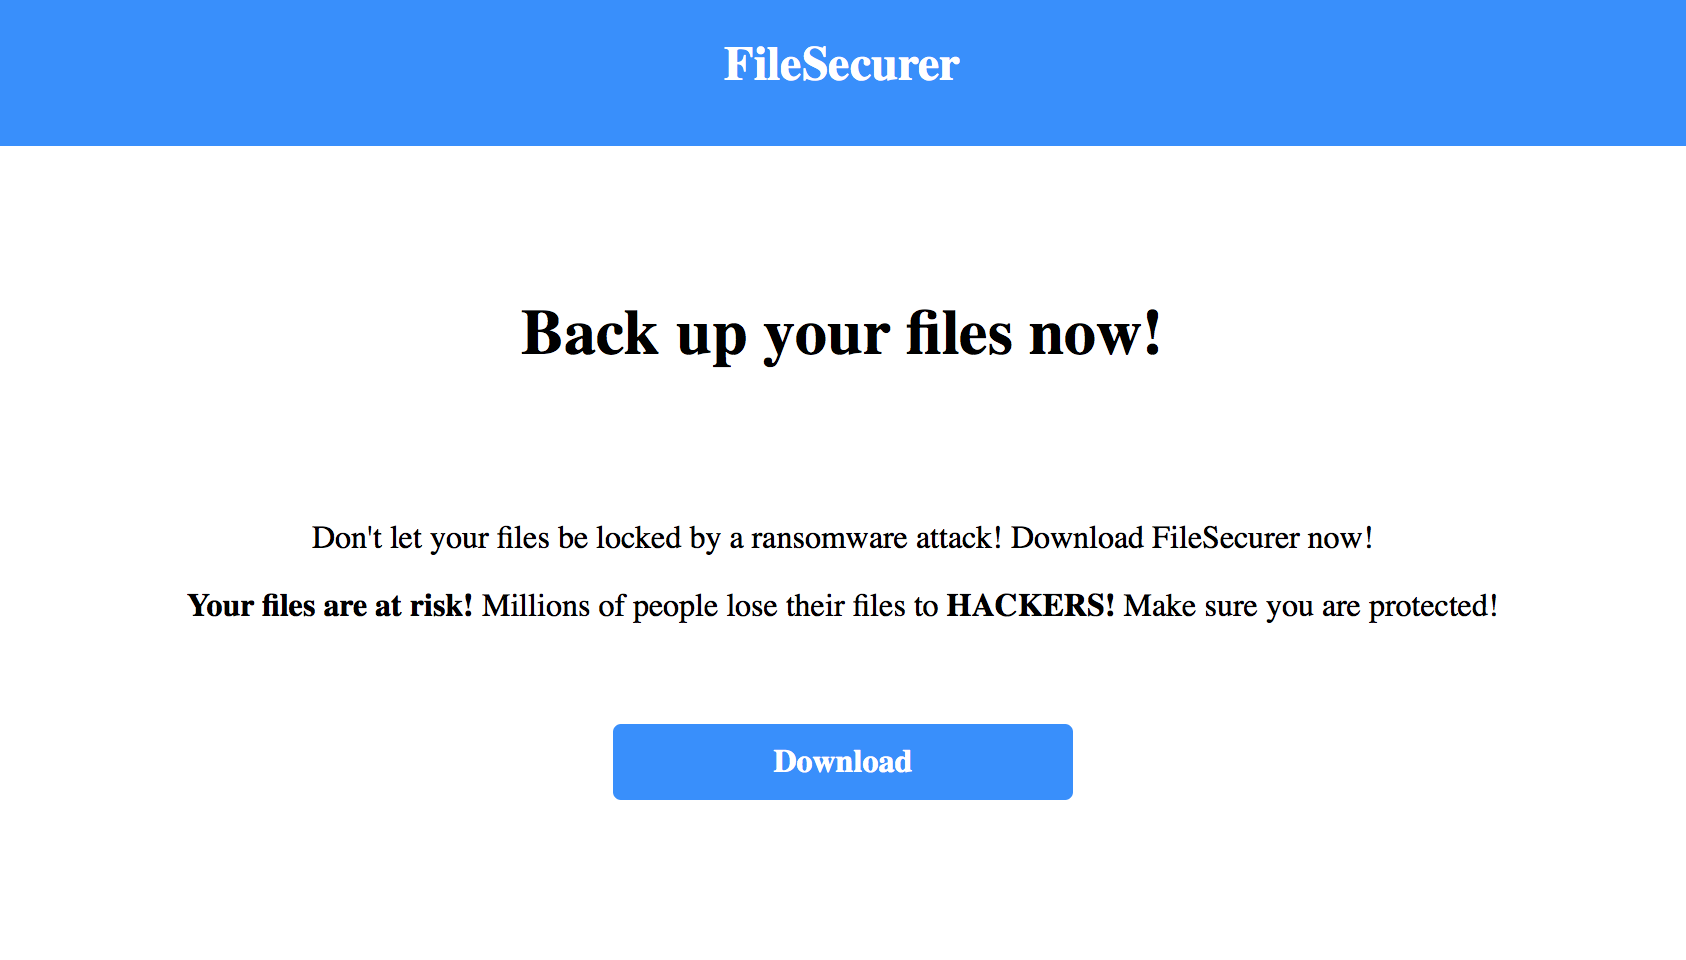
\includegraphics[width=9cm]{phishing}
      \caption{MrRansom phishing email}
      \label{fig:mrransom-phishing}
    \end{figure}

    Distributing the malware is often the most problematic part of building ransomware, most of the time you have to convince and/or trick a victim into downloading and executing the malware. Phishing emails are a hugely popular attack vector, as shown by \cite{ramzan2007phishing} \textit{“In 2006 Symantec’s Brightmail system blocked 2,848,531,611 phishing emails”}. As shown in figure \ref{fig:mrransom-phishing}, MrRansom utilises this attack vector by convincing the victim to download backup software to help them avoid a ransomware attack.

  \subsection{Obfuscation}
    Once the victim has downloaded the payload, it needs to look trustworthy enough that they actually run the file. A python module is typically run from the command line so this would not be good enough for the average user. To get around this, the python module could be compiled into a single executable file which can be just click-to-run. This could be achieved using a packager such as Pyinstaller (\url{http://www.pyinstaller.org}).

  \subsection{Command and Control (C\&C) Communications}
    The command and control server for this ransomware is very simple. It's only purpose is to catalogue the keys sent by the target machines. It does this by simply saving the recieved key into a file and uses the sender's ip address as the file name.

    Before the encryption begins on the target machine, it uses the python random module to generate a 32 bit random number which is used as the base key. Before the program actually starts encrypting files it attempts to send this key to the command and control server, but if it is unable to recieve an OK (HTTP 200) response, the program prints an error to the console and quits. This is due to the fact that the key should not be kept on the local machine due to the possibility of it being found and used to decrypt the files before payment has been made.

    The server is needed in order for any victim to be able to decrypt their files. When they have paid their ransom and the mrransom module is run in decrypt mode, it polls the server in order to attempt to retrieve the decryption key. A quick check is made to determine if the correct key is recieved, as the ransomware stores the MD5 hash of the key in the specified encryption directory as a ‘ransom.pwnhash’ file. If the recieved key does not match this hash then the program prints an error to the console and quits.

  \subsection{Files to encrypt}
    The MrRansom application is able to encrypt any file, as defined in a ‘.json’ file provided with the payload. The default installation would encrypt critical personal files such as: .docx, .pdf, .txt, .xlsx, .csv, .jpg, .png etc. For an attack onto personal computers, these would be the most valuable and likely sentimental files on the victims machine, which are often not backed up therefore making them more likely to want to pay the ransom.

    The program is able to search through all files from a given root directory and make an in-memory list of them all. When the encryption process begins it then loops through each of these files and checks it against the list of file types to encrypt.

  \subsection{Encryption}
    \begin{figure}[ht]
      \centering
      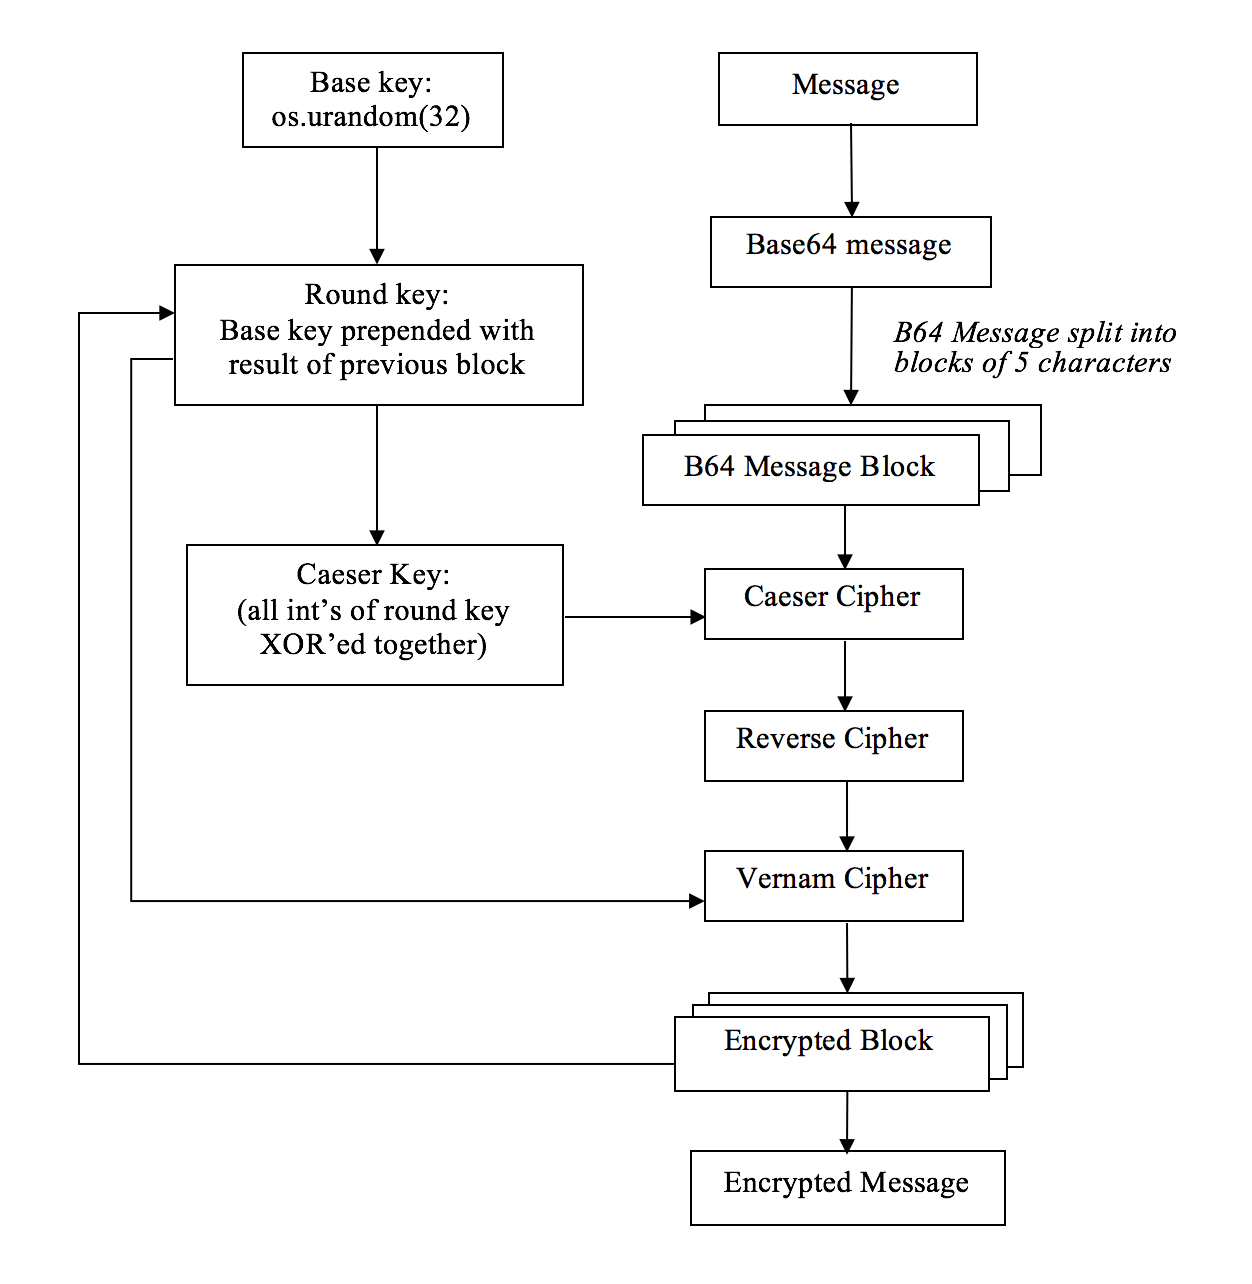
\includegraphics[width=9cm]{cipher-diagram}
      \caption{Product cipher component flow}
      \label{fig:cipher-diagram}
    \end{figure}

  % Yeah pretty much. But i was going to write about the potential for using executable packers/ email distribution and crypto wallet payments etc

  \subsection{Decryption}

  \subsection{Payment instructions}
    \begin{figure}[ht]
      \centering
      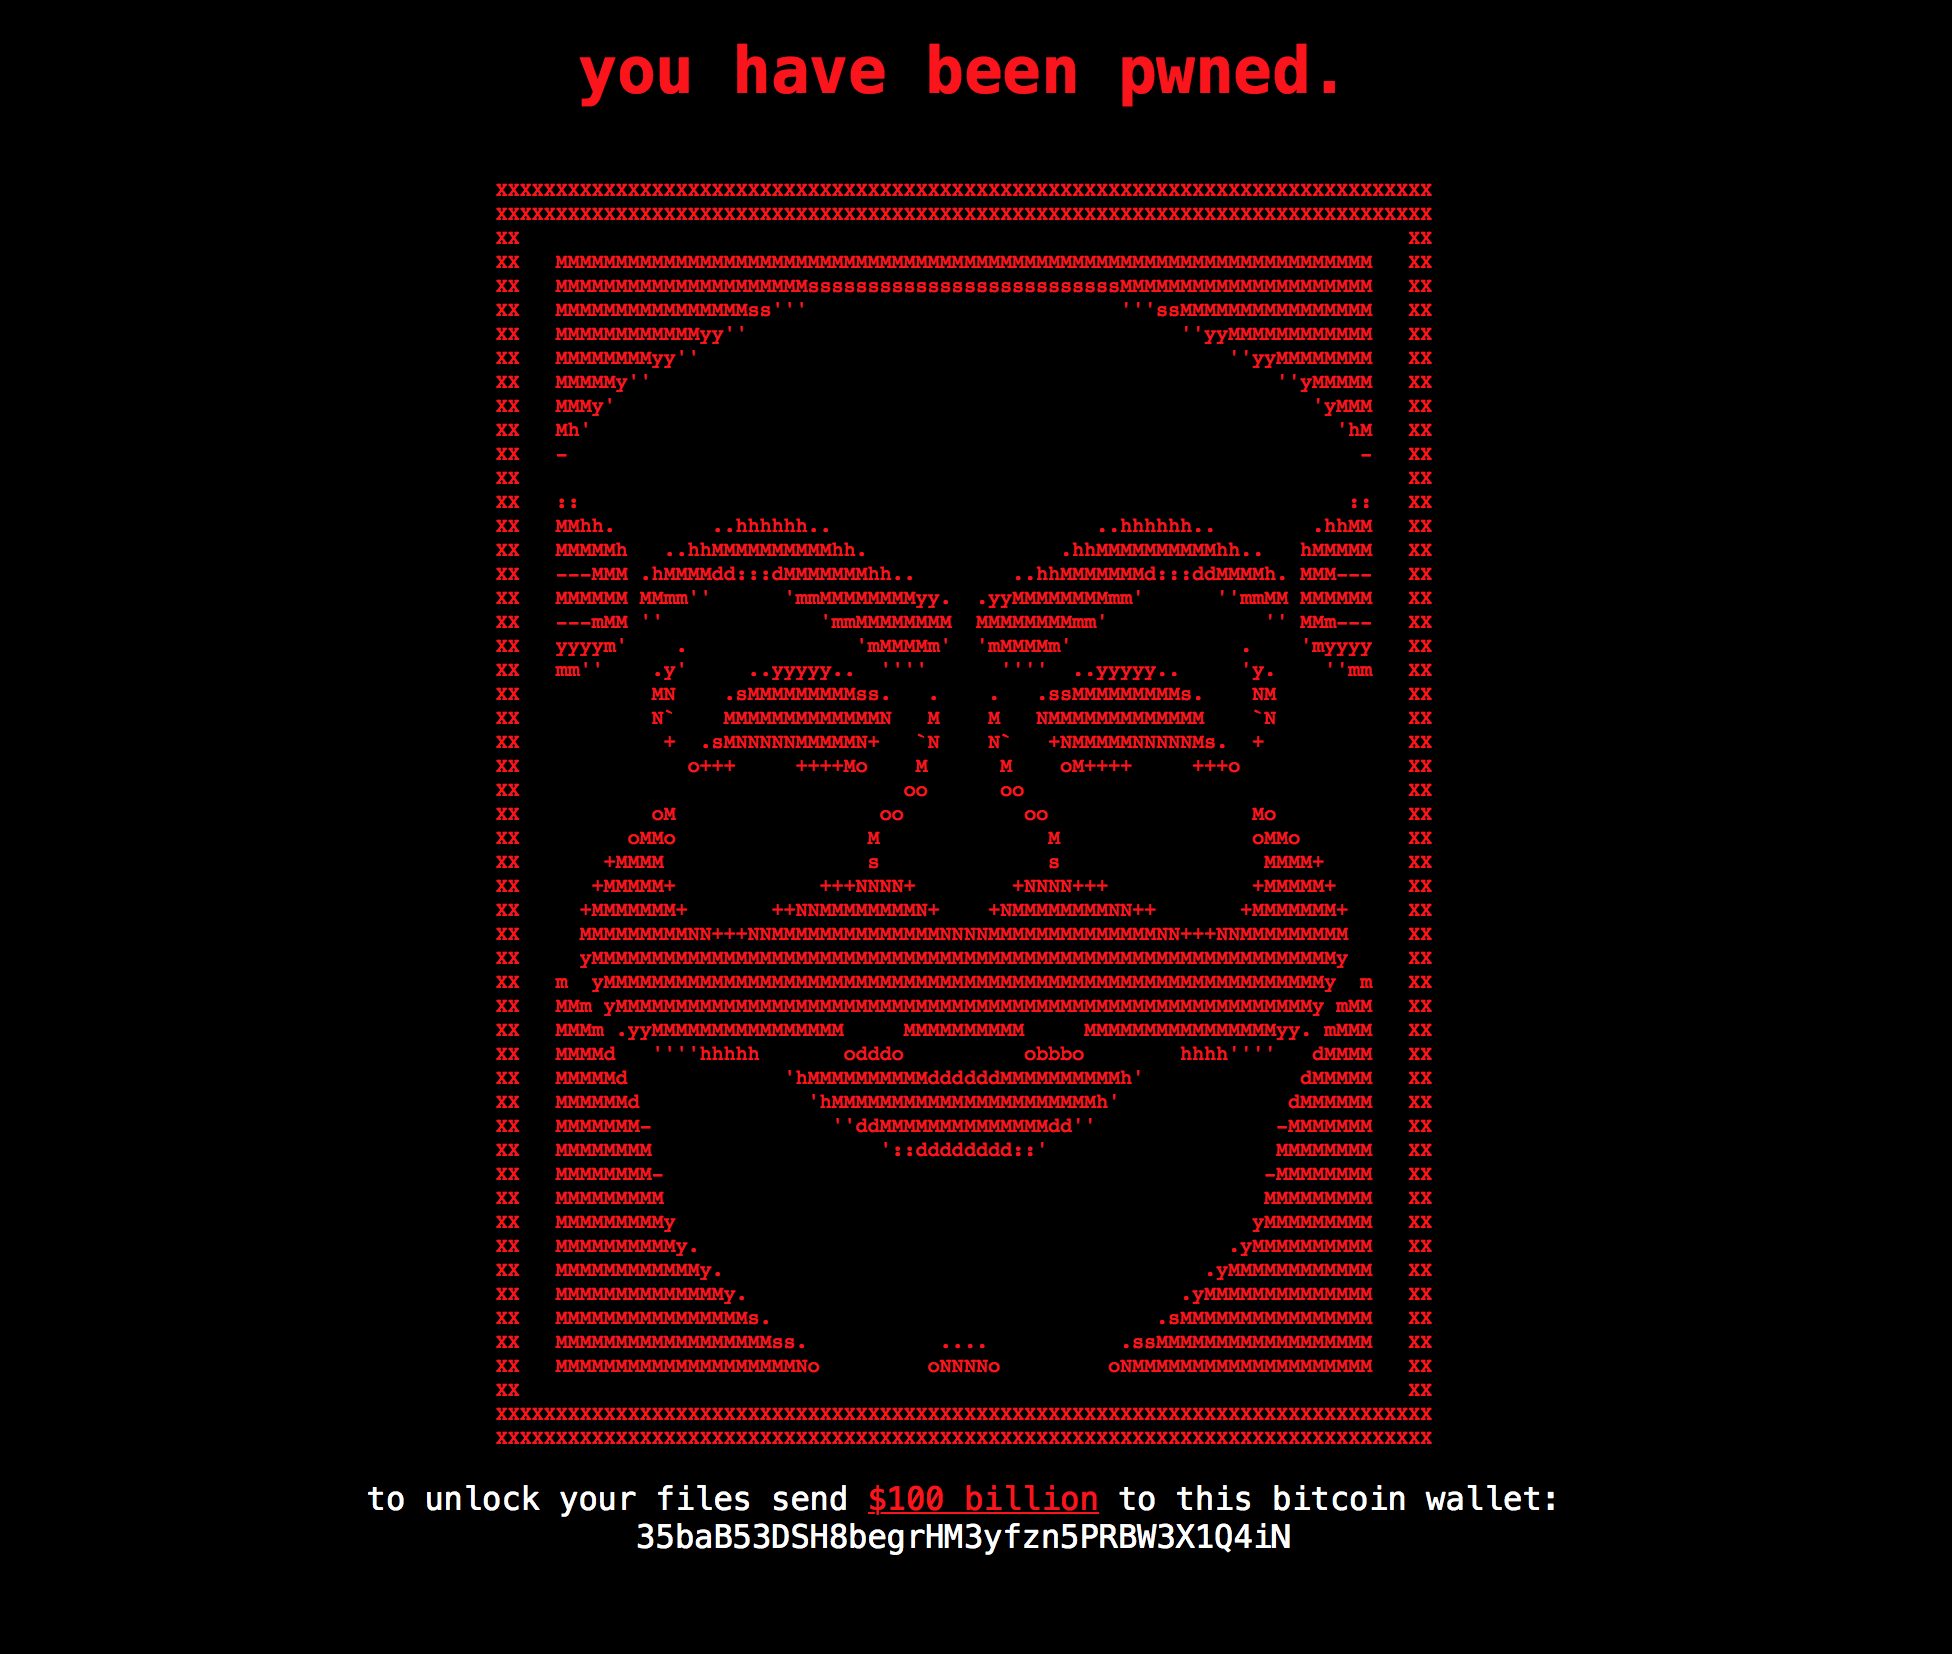
\includegraphics[width=9cm]{payment}
      \caption{MrRansom payment instructions}
      \label{fig:mrransom-payment-instructions}
    \end{figure}

    An html file (shown in Figure  \ref{fig:mrransom-payment-instructions}) is packaged with the mrransom module and once the encryption process has completed it copies the file to whichever root directory was specified for encryption, and then a python command opens that file in the default browser.

\newpage

\bibliographystyle{agsm}
\bibliography{mrransom-report}

\end{document}
